\documentclass{beamer}

\usepackage[utf8x]{inputenc}
\usepackage{default}
\usepackage{verbatim}
\usepackage{comment}
\usepackage{listings}  
\usepackage{algorithmic}
\usepackage{algorithm}
\usepackage{graphics}

%\usetheme{default}
\usetheme{Boadilla}

\title{Swarm Intelligence Seminar:\\Training Recurrent Neural Networks with Breeding Swarm}
\author{Xiwen Cheng \& Barry van Veen}
\institute{LIACS}
\date{\today}

\begin{document}

\begin{frame}
\titlepage
\end{frame}

\begin{frame}
\tableofcontents
\end{frame}

\section{Particle Swarm Optimizer}
\begin{frame}[fragile]
  \frametitle{Introduction: PSO}
  \begin{itemize}
    \item inspired by behavior of bird flocking
    \item population based stochastic optimization technique
    \item proposed by Kennedy and Eberhart in 1995 
  \end{itemize}
  
  \bigskip
  \begin{itemize}
    \item population with particles (birds)
    \item particle represents solution in search space
    \item particle consists of position and velocity
    \item particles position is updated
  \end{itemize}

\end{frame}

\begin{frame}[fragile]
  \frametitle{Basic algorithm}
  \begin{algorithmic}
    \STATE $t \gets 0;$
    \STATE $randomly\: initialize\: V(t);$
    \STATE $randomly\: initialize\: P(t);$
    \STATE $evaluate\: P(t);$
    \STATE $update\: pBest;$
    \STATE $update\: nBest;$
    \REPEAT
      \STATE $V(t+1) \gets updateVelocity(V(t));$
      \STATE $P(t+1) \gets P(t) + V(t+1);$
      \STATE $evaluate\: P(t+1);$
      \STATE $update\: pBest;$
      \STATE $update\: nBest$
      \STATE $t \gets t + 1;$
    \UNTIL{$stop\: requirement$}
  \end{algorithmic}
\end{frame}

\begin{frame}[fragile] 
  \frametitle{Basic algorithm}
  \begin{tabular}{ll}
    $V(t+1) =$ 	& $w \times V(t)$ \\
		& $+ c_{1} \times rand_{1}() \times (pBest - P(t))$ \\
		& $+ c_{2} \times rand_{2}()\times (nBest - P(t))$ \\
    $P(t+1) =$	& $P(t) + V(t+1)$ \\
  \end{tabular}

  \bigskip
  \begin{tabular}{ll}
    $pBest$		& best solution found so far by a particle \\
    $nBest$		& best solution found by $n$ neighbourhood \\
    $w$			& inertia weight (damping weight) \\
    $c_1$, $c_2$	& social parameters \\
    $rand_1$, $rand_2$	& normal distributed random values \\
    $vMax$		& maximum velocity \\
  \end{tabular}
\end{frame}

\begin{frame}[fragile]
  \frametitle{Update function}
  \begin{figure}
   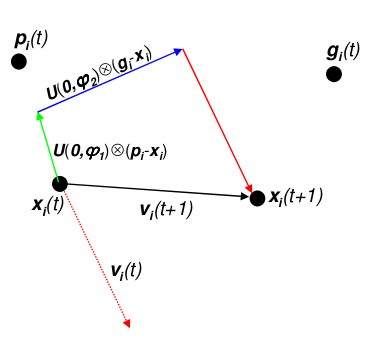
\includegraphics[scale=0.5]{pso}
   \caption{PSO update function}
  \end{figure}
\end{frame}

\begin{frame}[fragile]
  \frametitle{Modifications to the algorithm}
  \begin{itemize}
    \item discrete version
    \item multiobjective optimization
    \item constraint optimization
    \item dynamic environments
  \end{itemize}
\end{frame}

\begin{frame}[fragile]
  \frametitle{Applications of the algorithm}
  \begin{itemize}
    \item neural network training
    \item parameter optimization
    \item feature selection
    \item interaction with other algorithms
  \end{itemize}
\end{frame}


\section{Genetic algorithm}

\begin{frame}[fragile]
  \frametitle{Introduction: GA}
  \begin{itemize}
    \item inspired by evolution
    \item population based stochastic optimization technique
    \item proposed by Holland in 1970's
  \end{itemize}
  
  \bigskip
  \begin{itemize}
    \item population of bitstrings 
    \item bitstrings encode solutions
    \item individual is changed by crossover and mutation
    \item population is changed by creating offspring and selecting individuals
  \end{itemize}

\end{frame}

\begin{frame}[fragile]
  \frametitle{Basic algorithm}
  \begin{algorithmic}
    \STATE $t \gets 0;$
    \STATE $initialize\: P(t);$
    \STATE $evaluate\: P(t);$
    \REPEAT
      \STATE $P'(t) \gets select\mbox{-}mates(P(t));$
      \STATE $P''(t) \gets crossover(P'(t), p_c);$
      \STATE $P'''(t) \gets mutation(P''(t), p_m);$
      \STATE $evaluate\: P'''(t);$
      \STATE $P(t+1) \gets P'''(t);$
      \STATE $t \gets t + 1;$
    \UNTIL{$stop\: requirement$}
  \end{algorithmic}
\end{frame}

\begin{frame}[fragile]
  \frametitle{Operators}

  \begin{columns}[lT] % the "c" option specifies center vertical alignment
    \column{.5\textwidth} % column designated by a command
    \begin{itemize}
      \item Selection
      \begin{itemize}
	\item proportional
	\item tournament
      \end{itemize}
      \item Crossover
      \begin{itemize}
	\item single point
	\item uniform
	\item blended-$\alpha$
      \end{itemize}
      \item Mutation 
      \item Elitism
    \end{itemize}
    
    \column{.4\textwidth}
    \scriptsize
    \begin{verbatim}
      selection:
      0000000000
      1111111111

      crossover:
      0000011111
      1111100000

      mutation:
      1000011111
    \end{verbatim}
    
  \end{columns}

\end{frame}


\begin{frame}[fragile]
  \frametitle{Blended-$\alpha$ crossover}
  \begin{algorithmic}
    \STATE $select\: parents\: x(t), y(t);$
    \FOR{$i=1$ to $n$}
      \STATE $\delta_i \gets |x_i(t) - y_i(t)|;$
      \STATE $min_i \gets  min(x_i,y_i)$\\
      \STATE $max_i \gets max(x_i,y_i)$\\
      \STATE $u_x, u_y \gets$ uniform random number on interval $[min_i-\alpha \delta_i, max_i+\alpha \delta_i]$;
      \STATE $x_i(t+1) = u_x;$
      \STATE $y_i(t+1) = u_y;$
    \ENDFOR
  \end{algorithmic}
  
  \bigskip
  $\alpha$ was set to $0.1$ and \\
  Crossover rate was 0.6\\
\end{frame}

\begin{frame}[fragile]
  \frametitle{Comparison PSO / GA}
  \framesubtitle{Similarities}
  \begin{itemize}
    \item Population based
    \item Global search methods
    \item PSO update function performs actions similar to crossover, mutation
    \begin{itemize}
      \item Update is depending on $pBest$ and $nBest$ and combines these two
      \item Update function has random factors to increase exploration
    \end{itemize}
  \end{itemize}
\end{frame}

\begin{frame}[fragile]
  \frametitle{Comparison PSO / GA}
  \framesubtitle{Differences}
  \begin{itemize}
    \item PSO has no selection mechanism, GA has selection and elitism
    \item PSO has directional updates, GA has omnidirectional mutation
    \item PSO mixes neighbours, GA mixes "random" individuals
    \item PSO is more ergodic than a GA
  \end{itemize}
\end{frame}

\section{Breeding Swarm}
\begin{frame}[fragile]
  \frametitle{Introduction: BS}
  Combining ideas of:
  \begin{itemize}
    \item PSO: velocity and position update rules
    \item GA: selection, crossover and mutation
  \end{itemize}
  
\end{frame}
\begin{frame}[fragile]
  \frametitle{Generic Hybrid Algorithm}
  \framesubtitle{Pseudo algorithm}
  \begin{algorithmic}
    \STATE $t \gets 0;$
    \STATE $initialize\: P(t), V(t);$
    \STATE $evaluate\: P(t);$
    \REPEAT
      \STATE $P_{elite}(t) \gets copyBest(P(t), N_{elite});$
      \STATE $P_{pso}(t) \gets select_1(P(t), (N - N_{elite}) * \Psi);$
      \STATE $V'(t) \gets updateVelocity(V(t), P_{pso}(t));$
      \STATE $P'_{pso}(t) \gets updatePosition(P_{pso}(t), V'_{pso}(t));$
      
      \STATE $P_{ga}(t) \gets select_2(P(t), (N - N_{elite}) * (1-\Psi));$
      \STATE $P'_{ga}(t) \gets crossover(P_{ga}(t), p_c);$
      \STATE $P''_{ga}(t) \gets mutation(P'_{ga}(t), p_m);$
      
      \STATE $P(t+1) \gets P_{elite} \cup P'_{pso} \cup P''_{ga};$
      \STATE $V(t+1) \gets V'(t);$
      \STATE $evaluate\: P(t+1);$
      \STATE $t \gets t + 1;$
    \UNTIL{$stop\: requirement$}
  \end{algorithmic}
\end{frame}
\begin{frame}
  \frametitle{Generic Hybrid Algorithm}
  \framesubtitle{Parameters}
  \begin{tabular}{ll}
  $ N $ & Number of individuals \\
  $ N_{elite} $ & Number of elites \\
  $ \Psi $ & \emph{Breeding ratio}, proportion that undergoes \\
  & breeding; [0.0:1.0]\\
  $ select_1, select_2 $ & Two selection methods, may be different\\
  $ p_c, p_m $ & Crossover rate and mutation rate respectively \\
  \end{tabular}
  \bigskip
  
\end{frame}
\begin{frame}
  \frametitle{Breeding Swarm Algorithm (Settles \& Soule)}
  \framesubtitle{Flow}
  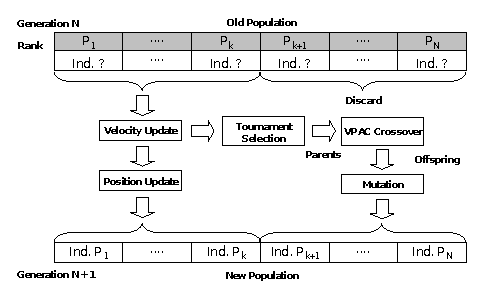
\includegraphics[scale=1.2]{bs}
\end{frame}

\begin{frame}[fragile]
  \frametitle{Breeding Swarm Algorithm (Settles \& Soule)}
  \framesubtitle{Parameters}
  Designed such that:
  \begin{itemize}
    \item GA performs global search
    \item PSO performs local search
  \end{itemize}
  \bigskip
  Standard velocity and position update rules are used. However: \\
  \begin{tabular}{ll}
  $N_{elite}$ & $ = 0$\\
  $\Psi$ & $ = 0.5, $ even distribution between PSO and GA \\
  $select_1 = select_2 $ & $ = $ tournament selection with size of 2\\
  $crossover$ & $ = $ \emph{Velocity Propelled Averaged Crossover} \\
  $mutation$ & $ = $ Gaussian with mean 0 and variance reduced linearly \\
  & each generation from 1.0 to 0.0 \\
  $inertia \: weight$  & $ = $ reduced linearly each generation from 0.7 to 0.4 \\
  $social \: parameter$ & $ = 2$, $c1 \mbox{ and } c2$ in position update\\
  $V_{max} $ & $ = \pm 1$ \\
  \end{tabular}
\end{frame}
\begin{frame}
  \frametitle{Velocity Propelled Averaged Crossover (VPAC)}
  \begin{equation}
   c_1(x_i) = \frac{p_1(x_i) + p_2(x_i)}{2.0} - \varphi_1 p_2(v_i)
  \end{equation}
  \begin{equation}
   c_2(x_i) = \frac{p_1(x_i) + p_2(x_i)}{2.0} - \varphi_2 p_1(v_i)
  \end{equation}
  \bigskip
  \bigskip
  \begin{tabular}{ll}
  $c_1(x_i), c_2(x_i) $ & Positions of childrens in dimension $i$\\
  $p_1(x_i), p_2(x_i) $ & Positions of parents in dimension $i$\\
  $p_1(v_i), p_2(v_i) $ & Velocities of parents in dimension $i$\\
  $\varphi_1, \varphi_2 $ & Uniform random variable in [0.0:1.0]\\
  \end{tabular}\\
  Increases diversity: accelerate away from parent's current direction
\end{frame}

\section{Training Recurrent Neural Network}
\begin{frame}[fragile]
  \frametitle{Artificial Neural Network}
  \begin{itemize}
    \item Inspired by Biological neurons
    \item Universal approximators for non-linear functions
    \item Consists of many layers: an input, multiple hidden and an output
  \end{itemize}
  \begin{columns}
  \begin{column}{0.4\textwidth}
  \begin{figure}
   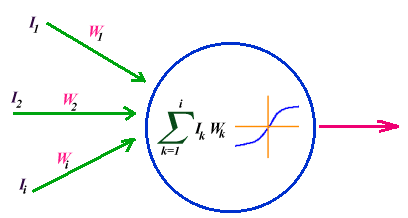
\includegraphics[scale=0.3]{neuron}
   \caption{Single neuron}
  \end{figure}
  \end{column}
  \begin{column}{0.6\textwidth}
  \begin{figure}
   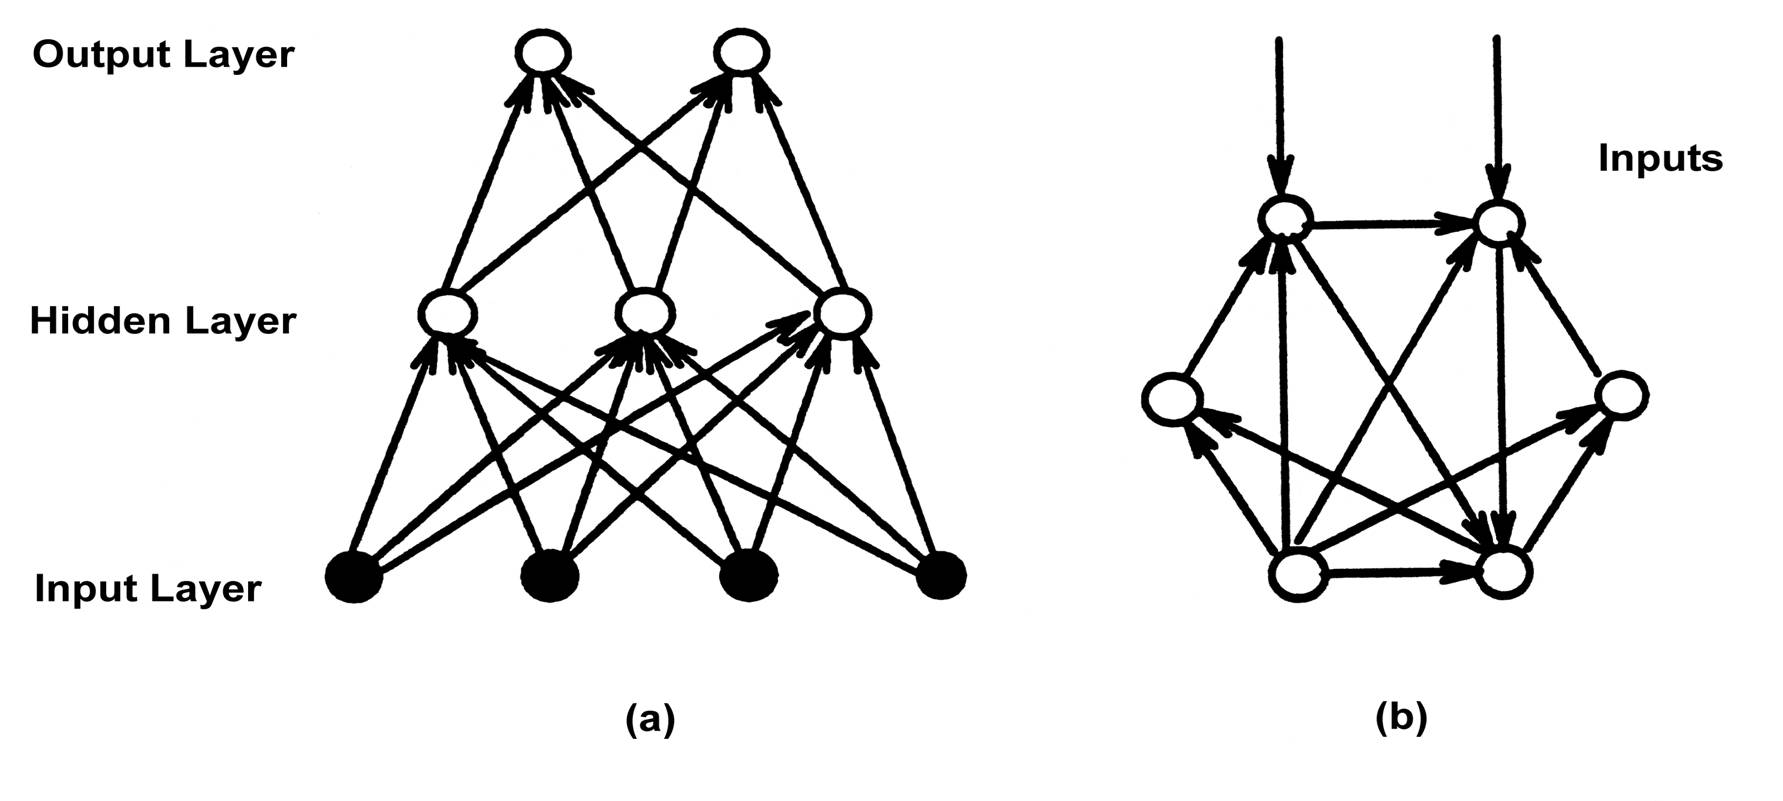
\includegraphics[scale=0.3]{nn}
   \caption{Feedforward and Hopfield (RNN)}
  \end{figure}
  \end{column}
  \end{columns}

\end{frame}
\begin{frame}[fragile]
  \frametitle{Recurrent Neural Network}
  We're considering a \emph{discrete-times, multi-layered \mbox{and} strongly connected} recurrent neural network \\
  \begin{figure}
   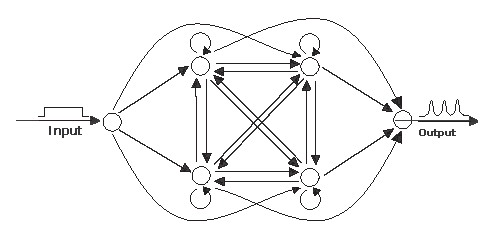
\includegraphics[scale=0.7]{strongrnn}
   \caption{Strongly connected RNN}
  \end{figure}
  Each node uses a symmetric sigmoidal activation function:
  \begin{equation}
   f(x) = \frac{2}{1+exp(-\beta x)} - 1
  \end{equation}
  Where $\beta = 1$ is the slope parameter
\end{frame}

\begin{frame}[fragile]
  \frametitle{Test problem}
  \begin{columns}
  \begin{column}{0.5\textwidth}
  \begin{figure}
   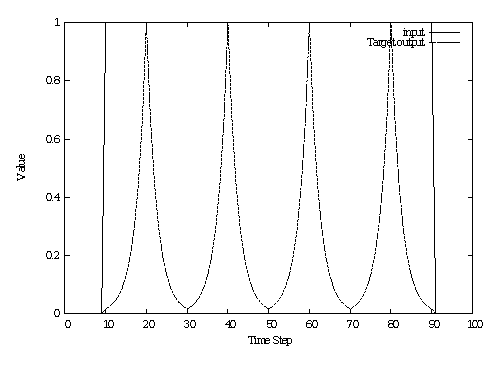
\includegraphics[scale=0.8]{targetrnn}
   \caption{Target: pulsed output signal}
  \end{figure}
  \end{column}
  \begin{column}{0.5\textwidth}
  Error function:\\
  $$E = \sum_{i=1}^{100}[(t_i-o_i)^2 + 2 \cdot (ts_i-os_i)^2]$$
  Where:\\
  \begin{tabular}{ll}
   $t_i$ & = target at time step $i$\\
   $o_i$ & = output at time step $i$\\
   $ts_i$ & = $t_i - t_{i-1}$ (target slope)\\
   $os_i$ & = $o_i - o_{i-1}$ (output slope)\\
  \end{tabular}\\
  \bigskip
  Slope component helps steer the training towards periodic behavior
  \end{column}
  \end{columns}
  
  
\end{frame}
\begin{frame}[fragile]
  \frametitle{Test parameters}
  \framesubtitle{Breeding Swarm}
  \begin{itemize}
    \item Training algorithms: GA, PSO and BS
    \item Network weight $w_i = \vec{x}_i \mbox{ where } \vec{x} \in P(t)$
    \item Dimensionality: $(LN)^2 + 2LN$ where $L$ is \#(layers) and $N$ is \#(nodes)/layer
    \item Networks with variety of hidden layers: 1-9
    \item Number of nodes per hidden layer: 1-9
    \item Per run: 2000 generations and 50 individuals
    \item 50 runs per network
    \item Initial weights are randomly selected from [-0.5, 0.5] range
    \item Velocity is restricted to [-1.0, 1.0], for PSO and BS
  \end{itemize}
\end{frame}
\begin{frame}[fragile]
  \frametitle{Results (1)}
  \begin{figure}
   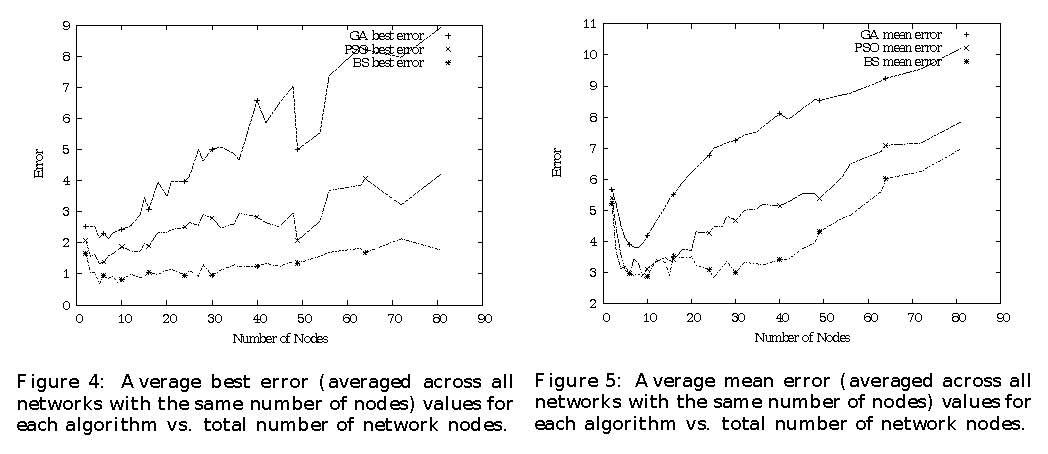
\includegraphics[scale=0.7]{results1}
  \end{figure}
\end{frame}
\begin{frame}[fragile]
  \frametitle{Results (2)}
  \begin{figure}
   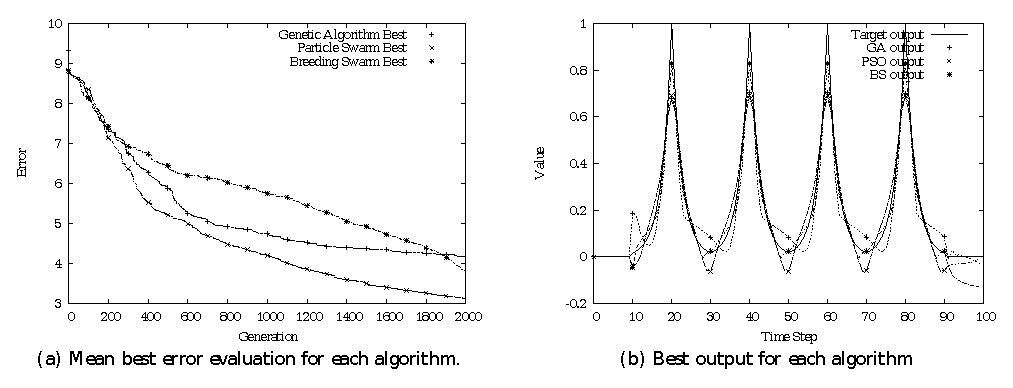
\includegraphics[scale=0.7]{results2}
   \caption{5 x 1 (35 weights)}
  \end{figure}
\end{frame}
\begin{frame}[fragile]
  \frametitle{Results (3)}
  \begin{figure}
   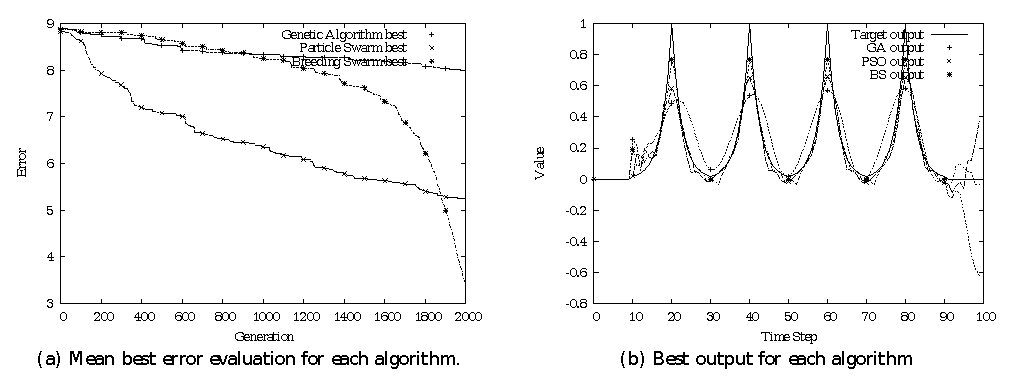
\includegraphics[scale=0.7]{results3}
   \caption{6 x 7 (1848 weights)}
  \end{figure}
\end{frame}
\begin{frame}[fragile]
  \frametitle{Results (4)}
  \begin{figure}
   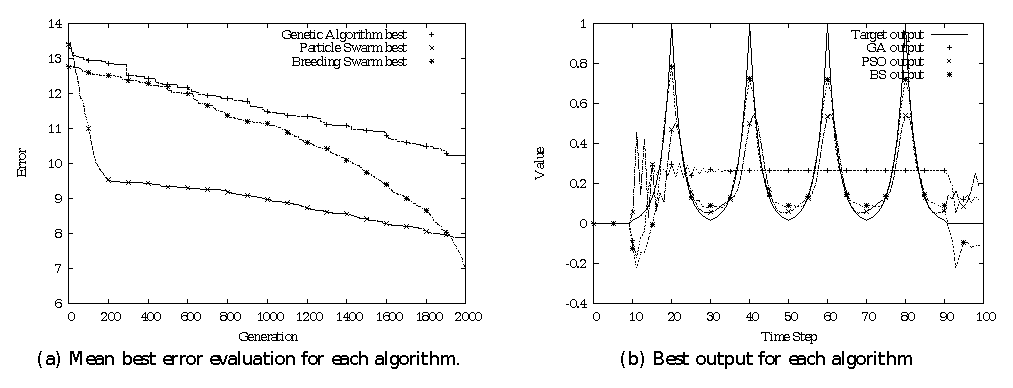
\includegraphics[scale=0.7]{results4}
   \caption{9 x 9 (6723 weights)}
  \end{figure}
\end{frame}


\section{Conclusions} 
\begin{frame}[fragile]
  \frametitle{Conclusions}
  Breeding swarm:
  \begin{itemize}
    \item scales well on large networks
    \item produces as good as or better results than GA and PSO in most cases
  \end{itemize}
\end{frame}

\begin{frame}[fragile]
  \frametitle{Discussion}
  \begin{itemize}
    \item In the BS articles non-standard versions of PSO and GA were used. Maybe these tests should be repeated with standard versions.
    \item The BS seems to perform good. What is still missing in the algorithm are self-adapting parameters.
    \item During the RNN training BS exhibits a remarkable behavior: Quickest improvements occur towards the end of the run.
    \item BS can evolve network topologies and weights simultaneously (VPAC).
  \end{itemize}
\end{frame}

\begin{frame}
 \frametitle{References}
 This presentation is based on the research done by \emph{Matthew Settles, Terrence Soule \mbox{and} Paul Nathan}. \\
 \bigskip
 The list of resources consulted are:
 \begin{itemize}
  \item Breeding Swarms: A GA/PSO hybrid -- \emph{M. Settles, T. Soule}
  \item Breeding Swarms: A New Approach to Recurrent Neural Network Training -- \emph{M. Settles, P. Nathan, T. Soule}
  \item Recent Advances in Particle Swarm -- \emph{X. Hu, Y. Shi, R. Eberhart}
  \item Comparison between Genetic Algorithms and Particle Swarm Optimization -- \emph{R. Eberhart, Y. Shi}
  \item Figures on NN were borrowed from the Neural Network Course, fall 2010.
  \item Figure on PSO update function was borrowed from the Natural Computing Course, fall 2010.
 \end{itemize}

\end{frame}

\end{document}
